
%\documentclass[mathserif]{beamer}
\documentclass[handout]{beamer}
%\usetheme{Goettingen}
%\usetheme{Warsaw}
\usetheme{Singapore}



%\usetheme{Frankfurt}
%\usetheme{Copenhagen}
%\usetheme{Szeged}
%\usetheme{Montpellier}
%\usetheme{CambridgeUS}
%\usecolortheme{}
%\setbeamercovered{transparent}
\usepackage[english, activeacute]{babel}
\usepackage[utf8]{inputenc}
\usepackage{amsmath, amssymb}
\usepackage{dsfont}
\usepackage{graphics}
\usepackage{cases}
\usepackage{graphicx}
\usepackage{pgf}
\usepackage{epsfig}
\usepackage{amssymb}
\usepackage{multirow}	
\usepackage{amstext}
\usepackage[ruled,vlined,lined]{algorithm2e}
\usepackage{amsmath}
\usepackage{epic}
\usepackage{epsfig}
\usepackage{fontenc}
\usepackage{framed,color}
\usepackage{palatino, url, multicol}
%\algsetup{indent=2em}
\newcommand{\factorial}{\ensuremath{\mbox{\sc Factorial}}}
\newcommand{\BIGOP}[1]{\mathop{\mathchoice%
{\raise-0.22em\hbox{\huge $#1$}}%
{\raise-0.05em\hbox{\Large $#1$}}{\hbox{\large $#1$}}{#1}}}
\newcommand{\bigtimes}{\BIGOP{\times}}
\vspace{-0.5cm}
\title{Natural Language Processing \\ Linear Models and Neural Networks}
\vspace{-0.5cm}
\author[Felipe Bravo Márquez]{\footnotesize
%\author{\footnotesize  
 \textcolor[rgb]{0.00,0.00,1.00}{Felipe Bravo-Marquez}} 
  
 

\date{\today}

\begin{document}
\begin{frame}
\titlepage


\end{frame}





\begin{frame}{Introduction to Neural Networks}
\begin{scriptsize}
\begin{itemize}
\item Very popular machine learning models formed by units called \textbf{neurons}.
\item A neuron is a computational unit that has scalar inputs and outputs. 
\item  Each input has an associated weight $w$.
 \item The neuron multiplies each input by its weight, and then sums them (other functions such as \textbf{max} are also possible). 
\item It applies an activation function $g$ (usually non-linear) to the result, and passes it to its output.
\item Multiple layers can be stacked.
\end{itemize}


\end{scriptsize}
\end{frame}


\begin{frame}{Activation Functions}

\begin{scriptsize}
\begin{itemize}
\item The nonlinear activation function $g$ has a crucial role in the network's ability to represent complex functions. 
\item Without the nonlinearity in g, the neural network can only represent linear transformations of the input.
\end{itemize}


\end{scriptsize}

\begin{figure}[htb]
	\centering
	 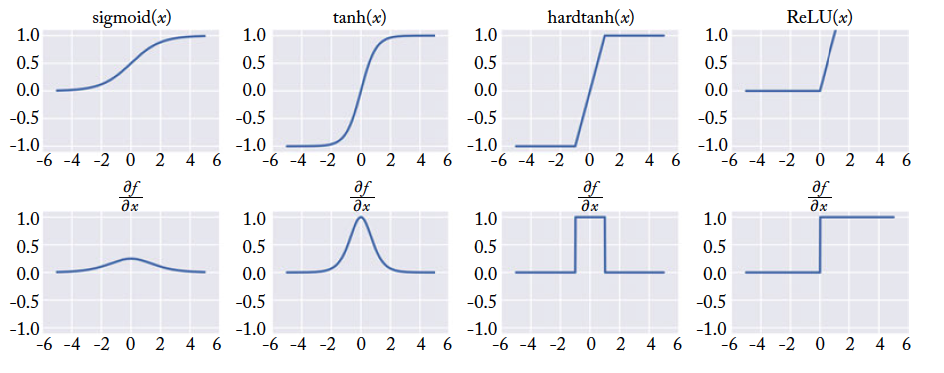
\includegraphics[scale=0.24]{pics/activations.png}
\end{figure}

\footnotetext{Source:\cite{goldberg2017neural}}

\end{frame}


\begin{frame}{Feedforward Network with two Layers}


\begin{figure}[htb]
	\centering
	 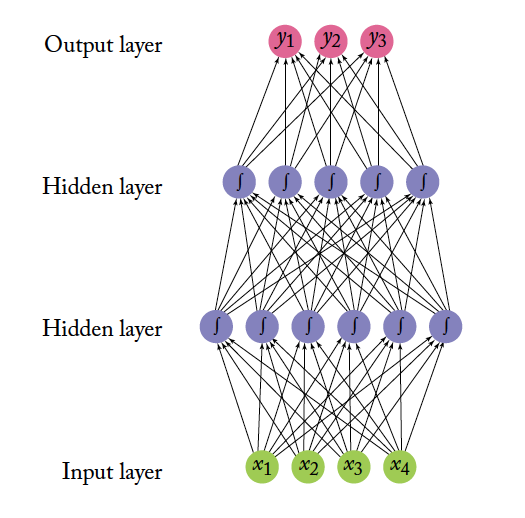
\includegraphics[scale=0.38]{pics/NN-example.png}
\end{figure}

\footnotetext{Source:\cite{goldberg2017neural}}

\end{frame}



\begin{frame}{Brief Introduction to Neural Networks}
\begin{scriptsize}
\begin{itemize}
\item The feedforward network from the picture is a stack of linear models separated by nonlinear functions.
\item The values of each row of neurons in the network can be thought of as a vector. 

\item The input layer is a 4-dimensional vector $(\vec{x})$, and the layer above it is a 6-dimensional vector $(\vec{h}^1)$.
\item The fully connected layer can be thought of as a linear transformation from 4 dimensions to 6 dimensions. 
\item A fully connected layer implements a vector-matrix multiplication, $\vec{h}=\vec{x}W$.
\item The weight of the connection from the $i$-th neuron in the input row to the $j$-th neuron in the output row is $W_{[i,j]}$.
\item The values of $\vec{h}$ are transformed by a nonlinear function $g$ that is applied to each value before being passed on as input to the next layer.

\end{itemize}

\footnotetext{Vectors are assumed to be row vectors and superscript indices correspond to network layers.}

\end{scriptsize}
\end{frame}





\begin{frame}{Brief Introduction to Neural Networks}
\begin{scriptsize}
\begin{itemize}
\item The Multilayer Perceptron (MLP) from the figure can be written as the following mathematical function:
\begin{center}
\begin{equation}
\begin{split}
NN_{MLP2}(\vec{x}) & =  \vec{y}  \\
\vec{h}^{1} &  = g^{1}(\vec{x}W^{1}+\vec{b}^{1}) \\
\vec{h}^{2} &  = g^{2}(\vec{h}^{1}W^{2}+\vec{b}^{2}) \\
\vec{y} &  = \vec{h}^{2}W^{3}\\
\vec{y} &  = (g^2(g^1(\vec{x}W^{1}+\vec{b}^{1})W^2+\vec{b}^2))W^3.\\
\end{split}
\end{equation}
\end{center}
%NN_{MLP2(x)}  =  y \\
%h^{1} = g^{1}(xW^{1}+b{1}) \\

\end{itemize}


\end{scriptsize}
\end{frame}







\begin{frame}{The Computation Graph Abstraction}
\begin{scriptsize}
\begin{itemize}
\item  One can compute the gradients of the various parameters of a network by hand and implement them in code.

\item This procedure is cumbersome and error prone.

\item For most purposes, it is preferable to use automatic tools for gradient computation [Bengio, 2012].

\item A computation graph is a representation of an arbitrary mathematical computation (e.g., a neural network) as a graph.

\item Consider for example a graph for the computation of $(a*b+1)*(a*b+2)$:

\begin{figure}[htb]
	\centering
	 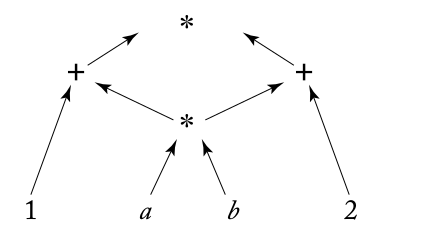
\includegraphics[scale=0.25]{pics/compGraph.png}
\end{figure}

\item The computation of $a*b$ is shared.

\item The graph structure defines the order of the computation in terms of the dependencies between the different components.

\end{itemize}
\end{scriptsize}
\end{frame}






\begin{frame}{The Computation Graph Abstraction}
\begin{scriptsize}
\begin{itemize}

\item  Te computation graph abstraction allows us to:


\begin{enumerate}
\begin{scriptsize}
 \item Easily construct arbitrary networks.
 \item Evaluate their predictions for given inputs (forward pass)
 
 \begin{figure}[htb]
	\centering
	 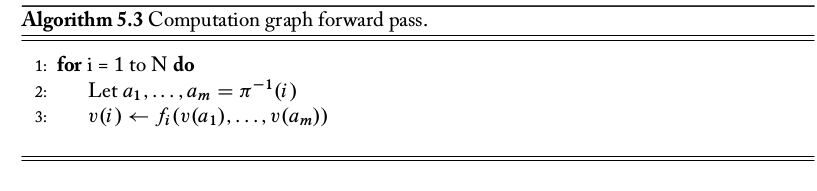
\includegraphics[scale=0.25]{pics/forwardPass.png}
\end{figure}

 
 
 \item Compute gradients for their parameters with respect to arbitrary scalar losses (backward pass or backpropagation).
 
 
  
 \begin{figure}[htb]
	\centering
	 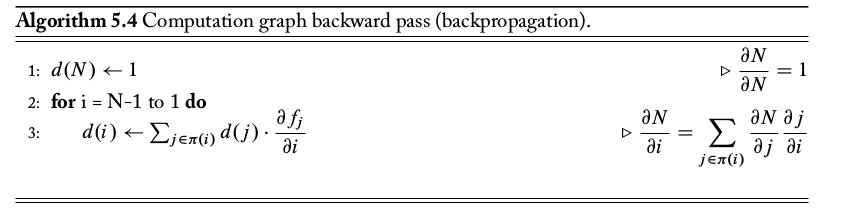
\includegraphics[scale=0.25]{pics/backwardPass.png}
\end{figure}
 
\end{scriptsize}
 \end{enumerate}
  
  
  
  
 \item The backpropagation algorithm (backward pass) is essentially following the chain-rule of differentiation\footnote{A comprehensive tutorial on the backpropagation algorithm over the computational graph abstraction: \url{https://colah.github.io/posts/2015-08-Backprop/}}.
 
  
\end{itemize}
\end{scriptsize}
\end{frame}


\begin{frame}{Deep Learning Frameworks}
Several software packages implement the computation-graph model. All these packages support all the essential components (node types) for defining a wide range of neural network architectures.
\begin{scriptsize}
\begin{itemize}
\item TensorFlow (\url{https://www.tensorflow.org/}): an open source software library for numerical computation using data-flow graphs originally developed by the Google Brain Team. 

\item Keras: High-level neural network API that runs on top of Tensorflow as well as other backends (\url{https://keras.io/}). 

\item PyTorch: open source machine learning library for Python, based on Torch, developed by Facebook's artificial-intelligence research group. It supports dynamic graph construction, a different computation graph is created from scratch for each training sample. (\url{https://pytorch.org/})


\end{itemize}
\end{scriptsize}
\end{frame}







\begin{frame}
\frametitle{Questions?}
%\vspace{1.5cm}
\begin{center}\LARGE Thanks for your Attention!\\ \end{center}



\end{frame}

\begin{frame}[allowframebreaks]\scriptsize
\frametitle{References}
\bibliography{bio}
\bibliographystyle{apalike}
%\bibliographystyle{flexbib}
\end{frame}  


%%%%%%%%%%%%%%%%%%%%%%%%%%%

\end{document}
